% PAQUETES
\documentclass[pdf]{beamer}
\usepackage[utf8]{inputenc}
\usepackage{beamer}
\usepackage[T1]{fontenc}
\usepackage[utf8]{inputenc}
\usepackage{helvet}
\usepackage{pstricks}
\usepackage{amssymb}
\usepackage{float}
\usepackage{multirow}
\usepackage{xcolor}
\usepackage{graphicx}
\usepackage{subfig}
\usepackage{hyperref}
\usepackage[ruled,,vlined,lined,linesnumbered,algosection]{algorithm2e}
\DeclareGraphicsExtensions{.epg,.pdf,.png,.jpg}%
\newcommand{\Rel}{\mathcal{R}}
\newcommand{\Sel}{\mathcal{S}}
\newtheorem{ejemplo}{Ejemplo}
\newtheorem{ejercicio}{Ejercicio}
\newtheorem{nada}{}

% DATOS INICIALES
\title{Título}
\author{Nombre Apellido}
\date{12/23/2023}

% INICIO DE DOCUMENTO
\begin{document}
    {
        \setbeamertemplate{navigation symbols}{}
        \begin{frame}[plain]
            \titlepage
        \end{frame}
    }
    
% TABLA DE CONTENIDOS
\begin{frame}{Contenido}
    \tableofcontents
\end{frame}


% SESIONES
\section{Introducción}
\label{sec:Introduccion}

\begin{frame}{Primera diapositiva}
Beamer es una clase de documento de LaTeX diseñada específicamente para crear presentaciones profesionales. Es una herramienta popular y poderosa que permite crear diapositivas con diferentes diseños, efectos de transición, animaciones y soporte para contenido matemático

\vspace{0.5cm}

Esto de aquí, es un \textbf{itemize}:

        \begin{itemize}
            \item Uno
            \item Fórmula matemática: \(H(X) = \mathbb{E}_X[I(x)] = -\sum_{x \in X} p(x) \log p(x)\)
            \item Otro ejemplo:
            \[
                f(n) \in O(g(n)) \Leftrightarrow \limsup_{n \rightarrow \infty} \frac{|f(n)|}{|g(n)|} < \infty
            \]
        \end{itemize}
        
\end{frame}
\begin{frame}
\frametitle{Colores}

\begin{nada}
Para usar colores hay que llamar el paquete 
{\color{blue!40!green} \textbackslash usepackage$\{xcolor\}$}.\\
\vspace{15px}
El comando es el siguiente:

\begin{center}

\fcolorbox{black}{blue!40!green}{ \color{white} $\{$\textbackslash color$\{magenta\}$ esto es una  prueba $\}$}\\

\textbf{}


\end{center}

\vspace{35px}
\textbf{Resultado: } {\color{magenta} esto es una prueba }
\end{nada}

\end{frame}
\begin{frame}{Items: Enumeración}

Como habíamos visto antes, un Itemize es una lista, no enumerada. Con \textbf{enumerate}, podemos hacer una lista enumerada. 

\begin{nada}
\textbf{Comando:}\\
\vspace{5px}

\textbackslash {\color{blue} begin}{\color{blue!40!green} $\{enumerate\}$}\\ \textbackslash {\color{blue} item[a)]} Item uno\\ \textbackslash {\color{blue} item[b)]} Item dos\\
\textbackslash {\color{blue} end}{\color{blue!40!green} $\{enumerate\}$}
\vspace{18px}\\
\textbf{Resultado:}\\
\begin{enumerate}
    \item[a)] Item uno 
    \item[b)] Item uno
\end{enumerate}

\end{nada}

\end{frame}
\begin{frame}{Secciones}
\section{Secciones y algortimos}
\label{sec:Secciones}

Las secciones se encuentran en la carpeta “sections”, la idea de esto es poder organizar de mejor manera cada sección del documento. Así se evita la gran cantidad de código en un solo archivo. En el archivo “main.tex” se encuentra únicamente los paquetes, portada, llamada de secciones y bibliografía.

Cada sección tiene un “label” que puede ser llamado así: \textbf{\ref{sec:Introduccion}}

\end{frame}
\begin{frame}{Imágenes}
\subsection{Imágenes}
\label{sec:imagenes}

A continuación se presenta un ejemplo de una imagen con respectivo caption. 

\vspace{1cm}

\begin{figure}[h!]
\centering

\includegraphics[scale = 0.1]{Imagenes/thumbnail_logo1.png}
\caption{Escudo UCR, sede Guanacaste}
\end{figure}

\end{frame}
\begin{frame}
\frametitle{Cuidado con el idioma}
\subsection{Idioma}
\begin{nada}
El idioma por defecto de \LaTeX es el inglés, por lo tanto al editar en español, debemos tener cuidado con tildes, letra ñ y otros símbolos.
\end{nada}
\begin{figure}[h!]
\centering
{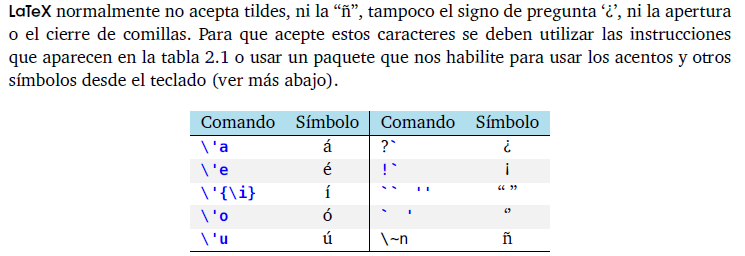
\includegraphics[scale=0.5]{Imagenes/imagen7}}
\end{figure}
\end{frame}
 \begin{frame}[fragile]
 \subsection{Código Java}

A continuación se presenta un ejemplo de como mostrar código de un lenguaje de programación.
 
  \frametitle{Ejemplo Java}
  \begin{verbatim}
import javax.swing.*;
Figura 1.8: Block.
   import java.awt.*;
   public class app_prg1 extends JApplet
   {
    public void init(){}
    public void paint ( Graphics g )
    {
     g.drawString(" 3 +46 = "+(3+46),30, 30 );
    }
}
\end{verbatim}
\end{frame}

\begin{frame}{Algoritmos}
\subsection{Algoritmos}

Los algoritmos se realzan con el paquete \textbf{algorithm2e}

\begin{algorithm}[H]
$a_0=y_0$\;
$s=\alpha_j-\alpha_0$\;
$f=x_j-x_0$\;
\For{$j=1$ \KwTo $m$
}{  $s=y_j-\alpha_0;\;$ $f=x_j-x_0$\;
\For{$k=1$ \KwTo $j-1$}
    {$s=s-\alpha_k \cdot f$\;
     $f=(x_j-x_k)\cdot f$\;
    }
    \Return $\alpha_j=s/f$ \;
}
\end{algorithm}

\textbf{{\footnotesize \url{https://tecdigital.tec.ac.cr/revistamatematica/Libros/LaTeX/MoraW_BorbonA_LibroLaTeX.pdf}}}

\end{frame}
\begin{frame}
\frametitle{Efecto}

Este efecto de transición es interesante, ya que nos presenta en un solo \textbf{itemize} los ítems de la lista que queremos mostrar. Sin embargo, al colocarles <\#número-> hace que cada ítem, se presente en una diapositiva diferente, dándonos el efecto de transición. 

\vspace{1cm}

\begin{itemize}
 \item<1-> Texto visible en la diapositiva 1
 \item<2-> Texto visible en la diapositiva 2
 \item<3-> Texto visible en la diapositiva 3
 \item<4-> Texto visible en la diapositiva 4
\end{itemize}

\end{frame}

%% FINAL
\begin{frame}
\Huge{\centerline{¡Muchas Gracias!}}
\end{frame}

\end{document}